\documentclass[11pt,a4paper]{article}

\usepackage[utf8]{inputenc} 
\usepackage[T1]{fontenc} 
\usepackage{lmodern}
\usepackage[margin=2cm]{geometry}
\usepackage[german]{babel}
\usepackage{array}
\setlength{\parindent}{0pt}
\setlength{\parskip}{1ex plus 0.5ex minus 0.5ex}

\usepackage{amsmath} 
\usepackage{graphicx} 
\usepackage{booktabs}
\usepackage[colorlinks]{hyperref}
\usepackage{nicefrac}
\usepackage{gensymb}
\usepackage[usenames,dvipsnames,svgnames,table]{xcolor}
\usepackage{multirow}
\usepackage{tikz}
\usepackage[section]{placeins}
\usepackage{wrapfig}

\hbadness=99999

\newcommand{\refpy}[1]{Siehe Anhang: \textit{Rechnungen in Python} (\texttt{{\color{incolor}In [{\color{incolor}#1}]}})}
\newcommand\dif{\mathop{}\!\mathrm{d}}
\newcommand{\halftime}[4]{\begin{figure}[h]
\begin{minipage}{.#1\textwidth}#3\end{minipage}\begin{minipage}{.#2\textwidth}
\centering
#4\end{minipage}
\end{figure}}
\newcommand{\pard}[2]{\frac{\partial #1}{\partial #2}}
\newcommand{\bigp}[1]{\bigg(#1\bigg)}

\renewcommand{\vec}{\boldsymbol}

\usepackage{etoolbox}

\makeatletter
\patchcmd{\@classz}
  {\CT@row@color}
  {\oldCT@column@color}
  {}
  {}
\patchcmd{\@classz}
  {\CT@column@color}
  {\CT@row@color}
  {}
  {}
\patchcmd{\@classz}
  {\oldCT@column@color}
  {\CT@column@color}
  {}
  {}
\makeatother

\newcommand{\rpm}{\raisebox{.2ex}{$\scriptstyle\pm$}}

\begin{document}

{
\centering 
\large 
Physiklabor für Anf\"anger*innen \\
Ferienpraktikum im Sommersemester 2018 \\[4mm]
\textbf{\LARGE 
Versuch 17: Trägheitsmomente/Steinerscher Satz
} \\[3mm]
(durchgef\"uhrt am 17.09.2018 bei Adrian Hauber)\\
Gruppe 14: Andréz Gockel, Patrick M\"unnich\\ 
\today \\[10mm]
}
%\vspace{88pt}
\vfill
\tableofcontents
\vfill
%\vspace{22pt}
%\listoffigures
%\vspace{22pt}
%\listoftables
\pagebreak

\section{Ziel des Versuchs}

Dieser Versuch hat drei Teile. Im ersten Teil wird mit Hilfe von einer Herleitung das Trägheitsmoment mit der Periodendauer in Zusammenhang gebracht, hiermit wird der Satz von Steiner überprüft.  

In dem zweiten Teil wird dann der theoretisch berechnete Wert verglichen mit dem experimentell bestimmten Wert. 

In dem dritten Teil wird mit einem Drehpendel der Zusammenhang von der Schwingungsdauer und dem Abstand von einer Zusatzmasse zum Mittelpunkt untersucht.
\section{Teil 1 - Herleitung der Schwingungsgelichung}

Der unterschied von einem mathematischen Pendel und einem physikalischen Pendels ist, dass es sich beim Physikalischen nicht um eine punktförmige Masse handelt, sondern der Schwerpunkt von einem starren Körper zur Rechnung verwendet wird, wobei das Trägheitsmoment berücksichtigt werden muss. Mit der rücktreibenden Kraft $F_r = -mg\sin\varphi$ und dem Abstand vom Aufhängepunkt zu Schwerpunkt $d$ können wir das Drehmoment ausdrücken als:
$$\vec{M} = -\vec{F_r} \times \vec{d} = dm\vec{g}\sin(\varphi)$$
mit der Kleinwinkelnäherung: $\sin\varphi \approx \varphi$:
$$\vec{M} = dm\vec{g}\varphi$$
Dies wird gleichgesetzt mit:
$$\vec{M} = \vec{\dot L} = - I \cdot \vec{\dot\omega} = - I \cdot \vec{\ddot\varphi}$$
$$\Rightarrow - I \cdot \vec{\ddot\varphi} = dm\vec{g}\varphi \quad \Rightarrow \vec{\ddot\varphi} = - \bigg(\underbrace{\frac{dmg}{I}}_{\omega^2}\bigg)\varphi \quad \Rightarrow \vec{\ddot\varphi} = - \vec\omega^2 \varphi$$
Mit $T = 2\pi \frac{1}{\omega}$ bekommt man: $T = 2\pi \sqrt{\frac{I}{dmg}}$.

Zunächst wird das Trägheitsmoment eines starren Körpers, in diesem fall von einem Stab (Vollzylinder) berechnet. Für das Trägheitsmoment bezüglich der Drehachse an einem Aufhängepunkt am ende des Stabes gilt:
$$I = \int \vec{r}_\perp^2 \dif m$$
mit $\dif m = \rho \dif V$und der Annahme, der Zylinder ist homogen, bekommt man: $$\displaystyle{I_{\textrm{Stab}} = \rho \int_V \vec{r}_\perp^2 \dif V}$$
Da nur der senkrechte Anteil zu der Drehachse des Ortsvektors einen Beitrag hat bekommen wir in Zylinderkoordinaten, mit $r$ als Radius und $l$ als länge:
$$I_{\textrm{Stab}_d} = \rho \int\displaylimits_{0}^{2\pi} \int\displaylimits_{0}^{l}\int\displaylimits_{0}^{r} r^3 \sin^2 \phi +rz^2 \dif r \dif z \dif\phi = \frac{1}{4} m r^2 + \frac{1}{3} m l^2 $$ 
Für einen Stab der durch den Mittelpunkt rotiert, wird die Integration zu:
$$I_{\textrm{Stab}_0} = \rho \int\displaylimits_{0}^{2\pi} \int\displaylimits_{\frac{-l}{2}}^{\frac{l}{2}}\int\displaylimits_{0}^{r} r^3 \sin^2 \phi +rz^2 \dif r \dif z \dif\phi = \frac{1}{4} m r^2 + \frac{1}{12} m l^2 $$
Aus dem Satz von Steiner ist zu erwarten, dass $I_{\textrm{Stab}_d} = I_{\textrm{Stab}_0} + md^2$ wobei $d$ der abstand vom  Schwerpunkt ist. Der abstand am ende des Stabes ist  $d = \frac{l}{2}$:
$$I_{\textrm{Stab}_d} = I_{\textrm{Stab}_0} + m\bigg(\frac{l}{2}\bigg)^2 = \frac{1}{4} m r^2 + \frac{1}{12} m l^2 + \frac{1}{4}ml^2 = \frac{1}{4} m r^2 + \frac{1}{3} m l^2$$
welches die Erwartung bestätigt.

Für die Drehscheibe dessen Rotationsachse parallel zur $z$-Achse ist, wird $\vec r_\perp^2$ in Zylinderkoordinaten zu $r^2(\underbrace{\sin^2\phi + \cos^2\phi}_{=1}) = r^2$ woraus das Integral
$$I_{\textrm{Scheibe}} = \rho \int\displaylimits_{0}^{2\pi} \int\displaylimits_{0}^{l}\int\displaylimits_{0}^{r} r^3 \dif r \dif z \dif\phi = \frac{1}{2}mr^2$$
ergibt.

\section{Teil 2 - Physikalisches Pendel}
\subsection{Aufbau}
\begin{wrapfigure}[14]{h}{0.4\textwidth}
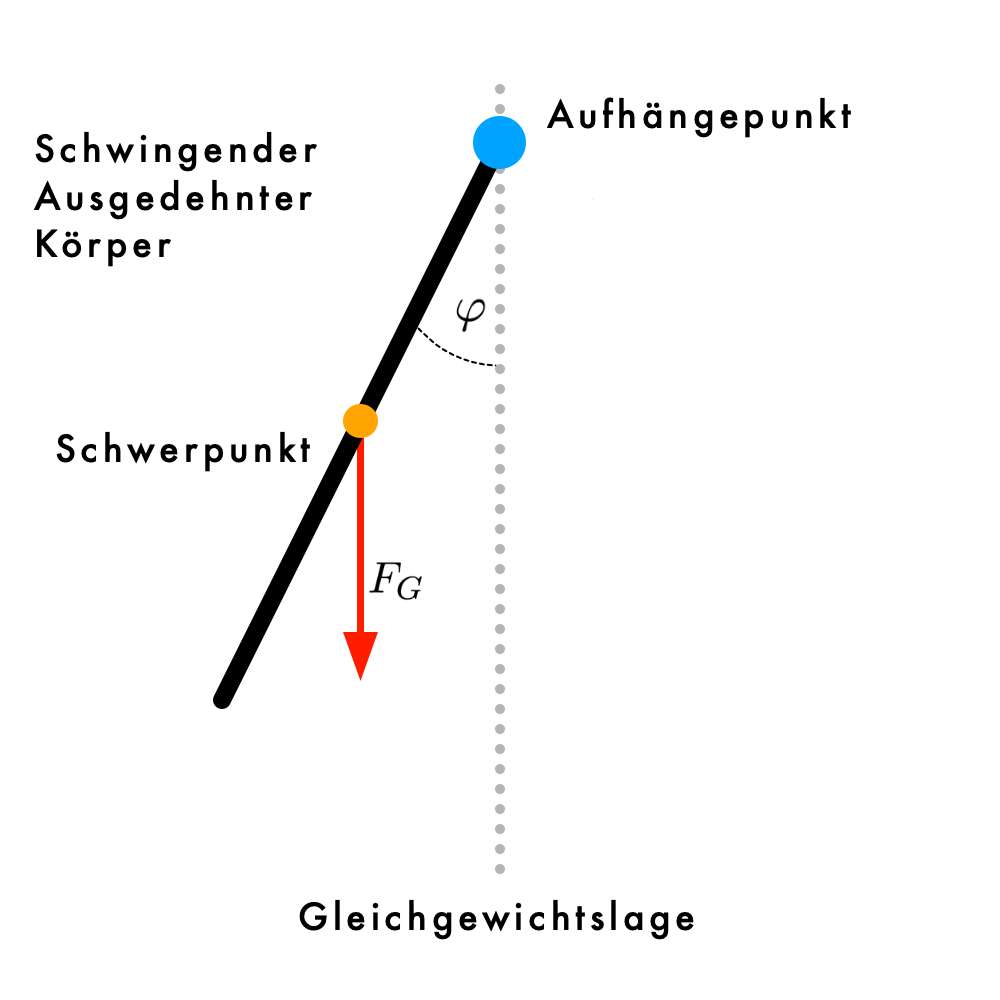
\includegraphics[width=0.4\textwidth]{Spend}
   %\renewcommand\thefigure{B1}
\caption{Versuchsaufbau 1}
\label{JS1}
\end{wrapfigure}

Um diesen Versuchsteil zu durchzuführen wird ein zylindrischer Stab der an einem Stativ gehängt werden kann verwendet. Zusätzlich werden ein Bandmass, Messschieber und eine Stoppuhr für die Messungen benötigt. 



\FloatBarrier
\subsection{Durchführung}

Zuerst wurde die Länge des Stabes mittels Bandmass gemessen. Daraufhin wurde mit dem Messschieber den Durchmesser des Stabes gemessen. Dann wurde der Stab an das Stativ gehängt und per hand zum Pendeln gebracht. Es wurde mit der Stoppuhr 30 mal eine Periode zeitlich gemessen. Danach wurde einmal 30 Perioden gemessen, um zu schauen welches verfahren ein kleineren Fehler hat. Der Fehler war etwas kleiner bei dem einmal messen von 30 Perioden.

\subsection{Auswertung}

\begin{table}[ht]
\caption{Bestimmte Werte (Teil 2)}
$$
\begin{array}{lr}
	\toprule 
	\textrm{Stablänge} & l = 96.7(3)\,\textrm{cm} \\
	\textrm{Radius} & r = 0.50(1)\,\textrm{cm} \\
	\textrm{Stablänge bis zum Aufhängepunkt} & a = 95.6(3)\,\textrm{cm}\\
	\textrm{Abstand Aufhängepunkt zu Schwerpunkt} & d = 49.5(5)\,\textrm{cm}\\
	\bottomrule 
\end{array}
$$
\end{table}
Wobei $d$ mit $d = \frac{l}{2} - (l - a)$ berechnet wurde.
Zuerst wird mit den obigen Herleitungen der theoretische Wert bestimmt. Mit $T = 2\pi \sqrt{\frac{I}{dmg}}$, und dem Einsetzen von $I_{\textrm{Stab}}$ bekommt man:
$$T = 2\pi \sqrt{\frac{\frac{1}{4} m r^2 + \frac{1}{3} m l^2}{dmg}} = 2\pi \sqrt{\frac{\frac{1}{4} r^2 + \frac{1}{3} l^2}{dg}}$$

mit $|g|=9.802\dots$\,$\nicefrac{\textrm{m}}{\textrm{s}^2}$\footnote{Dieser Wert wurde in einem anderen Versuch (Einleitungsversuch) bestimmt.} ist der theoretische Wert $T_0 = 1.593(5)$\,s wobei die Unsicherheit $\Delta T = 0.005$\,s mit der Gaußschen Fehlerfortpflanzung gefunden wurde:
$$\Delta T = \sqrt{ \bigp{\pard{T}{r}\Delta r}^2 + \bigp{\pard{T}{l}\Delta l}^2 + \bigp{\pard{T}{d}\Delta d}^2 }$$

Der experimentell bestimmte Mittelwert für 30 einzelne Perioden ist $T_1 = 1.591$\,s mit der Standardabweichung $s_T = 0.05$\,s und der Standardabweichung des Mittelwerts $s_{\bar T} = 0.01$\,s. 

Der experimentell bestimmte Wert für eine Messung von 30 Perioden ist $T_2 = 1.594\,$s mit der Unsicherheit von der Gesamtzeit $u_T = \pm0.3$\,s woraus die Unsicherheit $\frac{u_T}{\sqrt{n}} = 0.05$\,s der einzelnen Perioden kommt.

Also sind die drei Werte für die Schwingungsdauer:
$$T_0 = 1.593(5)\,\textrm{s} \qquad T_1 = 1.59(1)\,\textrm{s} \qquad T_2 = 1.59(5)\,\textrm{s}$$

\subsection{Diskussion}
\subsubsection{Fehleranalyse}

In diesem Versuchsteil wurde Hauptsächlich die Stoppuhr für die Periodendauer verwendet. Diese hat eine Unsicherheit von $\pm0.3$\,s da es von einem Menschen bedient wird und dessen Reaktionszeit einberechnet werden muss. Zusätzlich wurde ein Massband verwendet dessen Unsicherheit bei $\pm0.03\,$cm liegt da der Ansatz und Ablesepunkt sehr genau angelegt werden müssen. Ein Messschieber wurde auch verwendet um den Durchmesser des Stabes zu bestimmen, dies hat dank des Nonius eine sehr kleine Unsicherheit von $\pm0.1\,$mm. 

Ein systematischer Fehler ist der Energieverlust der durch die Reibung am Aufhängepunkt entsteht. Da die Reibung nur an einer sehr kleinen Fläche auftritt ist dieser Energieverlust verhältnismäßig klein. Andererseits sollte die Luftreibung größer sein da die zur Bewegung senkrechte Fläche wesentlich größer ist, jedoch bewegt sich der Stab nur langsam und sollte die Werte nicht all zu stark beeinflußen.

\subsubsection{Werte Vergleich}
 
\begin{align*}
	\textrm{Theoretische Wert} \quad & T_0 = 1.593(5)\,\textrm{s}\\
	\textrm{30 Einzelmessungen} \quad & T_1 = 1.59(1)\,\textrm{s}\\
	\textrm{Eine Messreihe} \quad & T_2 = 1.59(5)\,\textrm{s}
\end{align*}

Mit der Formel 
$$t = \frac{|T_a-T_b|}{\sqrt{\Delta T_a^2 + \Delta T_b^2}}$$
wird die Verträglichkeit der Werte berechnet. Wird der theoretische Wert mit den 30 Einzelmessungen verglichen bekommt man $t \approx 0.27$. und für den Vergleich von dem theoretischen Wert mit der Messreihe von 30 Perioden bekommt man $t \approx 0.06$. Diese Werte sind offensichtlich sehr verträglich. Obwohl der Fehler der 30 Einzelmeinungen kleiner ist liegt dieser Wert (minimal) weiter von dem theoretischen Wert, aus diesem Grund haben wir uns in Teil 3 für eine Messreihe von 30 Perioden entschieden. 

\pagebreak

\section{Teil 3 - Drehpendel}

\subsection{Aufbau}

\halftime{5}{5}{Zu diesem Versuch wurde ein Drehpendel verwendet, der aus einer Zusatzmasse, Drehtisch und einer Spiralfeder besteht. Die Zusatzmasse kann in verschiedenen Abständen von dem Mittelpunkt befestigt werden. Für die Messungen wurde eine Stoppuhr und ein Messschieber verwendet.}{
\centering
\fbox{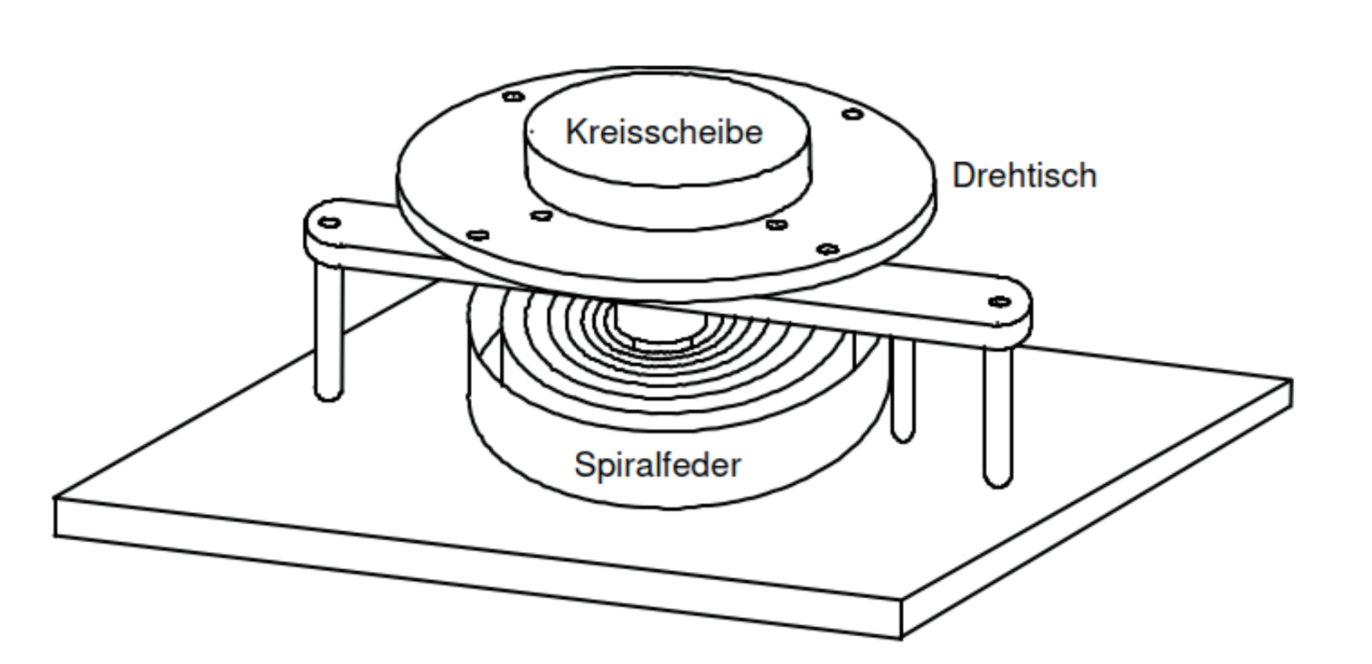
\includegraphics[width=0.7\textwidth]{Drehp}}
   \renewcommand\thefigure{B2}
\caption[Versuchsaufbau 2]{Versuchsaufbau 2 \cite{Anleitung}}
\label{B2}
}

\subsubsection{Durchführung}

Es wurden Breite und Durchmesser der Zusatzmasse mit dem Messschieber gemessen. (Die Masse wurde schon vorher bestimmt und auf das Pendel oben drauf Geschrieben.) Zunächst wurde die Zeit für 30 Perioden ohne Zusatzmasse gemessen. Danach wurde die Masse in den Mittelpunkt gesetzt und  derDrehtisch wurde von Hand soweit aus gelenkt, dass 30 Perioden zeitlich gemessen werden konnten. Dies wurde wiederholt für 10 Perioden. Anschliessend wurde die Masse mit einem Abstand von 15\,mm versetzt und wieder jeweils 30 und 10 Perioden gemessen. Diese Messung wurde wiederholt für vier weitere Abstände. 

\subsection{Auswertung}

\begin{table}[ht]
\caption{Relevante Werte (Teil 3)}
$$
\begin{array}{ll}
	\multicolumn{1}{l}{\textrm{Zu Bestimmende Werte}} \\
	\toprule 
	\textrm{Zusatzmasse} & m = 1.109(5)\,\textrm{kg} \\
	\textrm{Durchmesser} & d = 118.9(1)\,\textrm{mm} \\
	\textrm{Breite} & h = 12.9(1)\,\textrm{mm} \\
	\bottomrule \\
	\multicolumn{2}{l}{\textrm{Bekannte Werte}} \\
	\toprule
	\textrm{Abstände} & a = 15.0\,\textrm{mm}\cite{Anleitung}\\
	\bottomrule 
\end{array}
$$
\end{table}

Der theoretische Wert für das Trägheitsmoment der Drehscheibe ist mit der Formel $I_{\textrm{Scheibe}} = \frac{1}{2}mr^2$:
$$I_{\textrm{Scheibe}} = 1.960(9)\times 10^{-3}\,\textrm{kg}\,\textrm{m}^2$$
Die Unsicherheit wurde mit $$\Delta I = I\sqrt{\bigg(\frac{\Delta m}{m}\bigg)^2 + \bigg(2\frac{\Delta r}{r}\bigg)^2}$$ berechnet. 
Um das Trägheitsmoment des Drehpendels zu berechnen wird mit dem Drehmoment $\vec M = -D\cdot \varphi$:
$$T = 2\pi \sqrt{\frac{I}{D}}\quad \Rightarrow \quad I = \frac{T^2}{4\pi^2}D$$
Verwendung von dem Steinerschen Satz $I_a = I_0 + ma^2$ ergibt:
$$\frac{T^2}{4\pi^2}D = I_0 + ma^2$$ 
\begin{equation}\label{req}
	\Rightarrow \quad T^2 = 4\pi^2 \frac{I_0}{D} + 4\pi^2 \frac{m}{D}a^2
\end{equation}

Eine lineare Regression aus den Messwerten $T^2$ und unterschiedlichen Abständen $a^2$ wurde in Abbildung \ref{t17} mit Mathematica durchgeführt. Die Gleichung der Ausgleichsgerade ist: $c+bx=4.19(4) + 500(20) x$ welches mit Gleichung \eqref{req} verglichen werden kann, woraus sich $b = 4\pi^2 \frac{m}{D} = 500(20)$ ergibt. Hiermit kann die Federkonstante berechnet werden: $D = 0.087(4)$\,$\nicefrac{\textrm{N}}{\textrm{m}}$. Der Fehler auf $D$ wurde mit der Gaußschen Fehlerfortpflanzung für den Spezialfall der division berechnet:
$$\Delta D = D\cdot \sqrt{\bigg(\frac{\Delta b}{b}\bigg)^2+\bigg(\frac{\Delta m}{m}\bigg)^2}$$
Mit diesem Wert kann zunächst das Trägheitsmoment des Drehpendels ohne Zusatzmasse berechnet werden. 
$$I_{\textrm{Drehpendel}} = \frac{T^2D}{4\pi^2} = 7.3(4)\times 10^{-3}\,\textrm{kg\,m}^2$$
Wobei $T^2$ der Mittelwert der Schwingung ohne Zusatzmasse ist. Die Unsicherheit wird mit: 
$$\Delta I = \sqrt{\bigg(\frac{T^2}{4\pi^2}\cdot \Delta D\bigg)^2 + \bigg( \frac{TD}{2\pi^2}\Delta T\bigg)^2}$$
berechnet.
Addiert man dies mit dem Trägheitsmoment der Zusatzmasse bekommt man das Trägheitsmoment des gesamten Aufbaus:
$$I_1 = 9.3(4) \times 10^{-3}\,\textrm{kg\,m}^2$$
Als nächstes wird für $T^2$ der Mittelwert mit der Masse im Mittelpunkt verwendet:
$$I_2 = 9.2(5) \times 10^{-3}\,\textrm{kg\,m}^2$$
Zuletzt wird für $T^2$ der Achsenabschnitt der Ausgleichsgerade verwendet:
$$I_3 = 9.3(4) \times 10^{-3}\,\textrm{kg\,m}^2$$

Als nächstes wird noch der mit dem Steinerschen Satz berechnete Wert mit den Messwerten verglichen.

\begin{table}[h]
\caption{Berechnete und Gemessene Trägheitsmomente}
$$
\begin{array}{crr}
	\toprule 
	\textrm{Abstand} & \textrm{Berechnet} & \textrm{Gemessen}\\
	\textrm{[mm]} & \multicolumn{1}{c}{\textrm{[g\,m}^2]} & \multicolumn{1}{c}{\textrm{[g\,m}^2]}\\
	\midrule
	15.0 & 9.6(4) & 9.5(4)\\
	30.0 & 10.1(6) & 10.3(4)\\
	45.0 & 11.6(5) & 11.5(4)\\
	60.0 & 13.3(9) & 13.3(4) \\
	\bottomrule 
\end{array}
$$
\end{table}

\subsection{Diskussion}
\subsubsection{Fehleranalyse}
Bei diesem Versuch wurden wieder Stoppuhr, Messschieber und Massband verwendet, dessen statistische Fehler genau wie in Teil 2 sind. Das Gewicht der Zusatzmasse wurde vorgegeben und wir haben uns entschlossen eine Unsicherheit von $0.005\,$kg anzugeben, da wir nicht wissen wie sie gemessen wurde. 

Für diesen Teil haben wir uns für eine Messreihe von 30 Perioden entschieden. Wir haben eine weitere Messreihe von 10 Perioden gemessen da das Drehpendel wesentlich schneller as das Pendel verlangsamte. Für die jeweiligen Schwingungsdauern haben aus diesen zwei Messreihen den Mittelwert samt Fehler des Mittelwerts berechnet. 

Systematische Fehler wie in Teil 2 sind die Reibungskräfte. Die innere Reibung des Drehpendels schien wesentlich grösser zu sein als bei dem physikalischen Pendel, da es schneller verlangsamte. Die Luftreibung sollte kleiner sein da weniger Fläche senkrecht zur Bewegung ist, aber es drehte sich etwas schneller was Luftreibung stark beeinflusst. 

\subsubsection{Werte Vergleich}

\begin{align*}
	\textrm{Addition von Pendel und Masse} \quad & I_1 = 9.3(4) \times 10^{-3}\,\textrm{kg\,m}^2\\
	\textrm{Direkte Messung von Pendel mit Masse} \quad & I_2 = 9.2(5) \times 10^{-3}\,\textrm{kg\,m}^2\\
	\textrm{Graphisch bestimmte Wert} \quad & I_3 = 9.3(4) \times 10^{-3}\,\textrm{kg\,m}^2
\end{align*}

Die Addition von dem Trägheitsmoment mit dem der Masse ergibt genau den gleichen Wert wie die mit dem Achsenabschnitt berechnete Wert, und mit der gleichen Unsicherheit, also sind diese werte offensichtlich kompatibel. Der Vergleich wird wieder mit 
$$t = \frac{|I_a-I_b|}{\sqrt{\Delta I_a^2 + \Delta I_b^2}}$$
berechnet. Die direkte Messung von dem gesamten Aufbau und den anderen Werten ergibt $t \approx 0.16$ also sind alle drei Werte sehr kompatibel. 

Die mit dem Steinerschen Satz berechneten Trägheitsmoment, und den gemessenen Trägheitsmomenten bei Verschiebung der Masse, sind auch sehr kompatibel zueinander. Dies erfüllt unsere Erwartungen von dem Steinerschen Satz. Ein Verbesserungsvorschlag wäre eine Pendel mit einem noch grösseren Durchmesser zu nehmen, um mehr abstände Messen zu können, dies würde eine Stärkere aussage über die Linearität des Steinerschen Satzes haben.

\vfill

\begin{thebibliography}{9}
 %\bibitem{Uncertainties}''Correlations between variables are automatically handled, which sets this module apart from many existing error propagation codes.'' - https://pythonhosted.org/uncertainties/
 \bibitem{Anleitung} Physikalisches Institut der Albert-Ludwigs-Universität Freiburg (Hrsg.) (08/2018): Versuchsanleitungen zum Physiklabor für Anfänger*innen, Teil 1, Ferienpraktikum im Sommersemester 2018.
 \end{thebibliography}

\pagebreak

\section{Anhang}

\begin{table}[h]
\caption{Messwerte (Teil 2)}
$$
\begin{array}{cccc}
	\toprule 
	\textrm{Abstand/mm} & \textrm{10 Perioden/s} & \textrm{30 Perioden/s} & \textrm{Mittelwert/s}\\ 
	\midrule
	\multicolumn{1}{l}{\textrm{Ohne Zusatzmasse}} & 18.1 & 54.6 & 1.82(1)\\
	\phantom{zz.}0 & 20.6 & 60.3 & 2.04(4)\\
	15.0 & 20.8 & 63.0 & 2.09(1)\\
	30.0 & 21.8 & 63.2 & 2.14(5)\\
	45.0 & 22.9 & 68.9 & 2.29(1)\\
	60.0 & 24.9 & 72.0 & 2.45(6)\\
	\bottomrule 
\end{array}
$$
\end{table}

\begin{figure}[h]
\centering
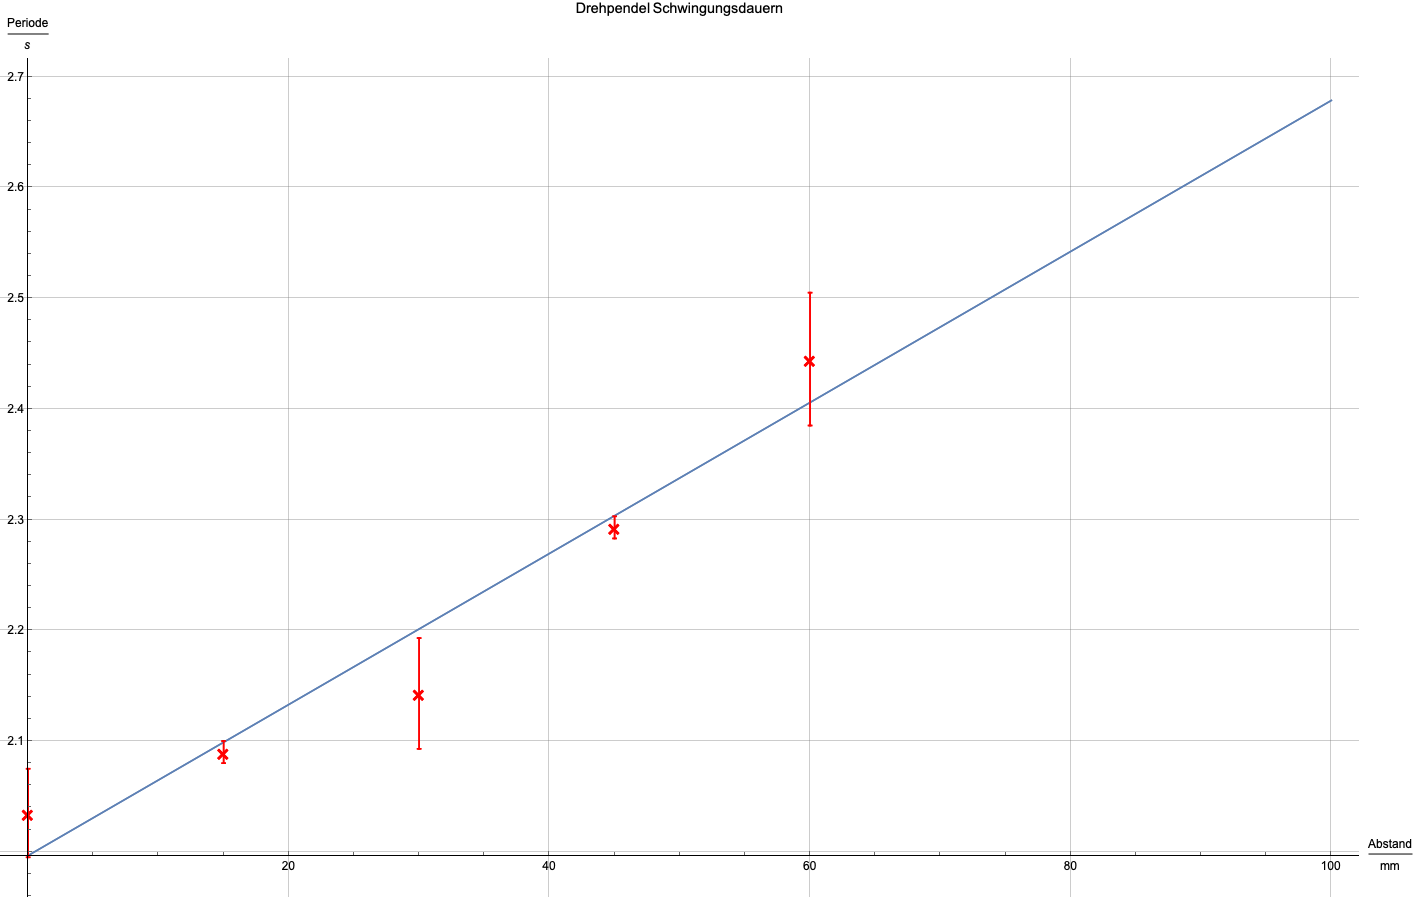
\includegraphics[width=1\textwidth]{trick17}
\renewcommand\thefigure{B3}
\caption{Mittelwerte}
\label{t17}
\end{figure}


\end{document}